\documentclass[12pt, titlepage]{article}

\usepackage{amsmath, mathtools}

\usepackage[round]{natbib}
\usepackage{amsfonts}
\usepackage{amssymb}
\usepackage{graphicx}
\usepackage{colortbl}
\usepackage{xr}
\usepackage{hyperref}
\usepackage{longtable}
\usepackage{xfrac}
\usepackage{tabularx}
\usepackage{float}
\usepackage{siunitx}
\usepackage{booktabs}
\usepackage{multirow}
\usepackage[section]{placeins}
\usepackage{caption}
\usepackage{fullpage}

\hypersetup{
bookmarks=true,     % show bookmarks bar?
colorlinks=true,       % false: boxed links; true: colored links
linkcolor=red,          % color of internal links (change box color with linkbordercolor)
citecolor=blue,      % color of links to bibliography
filecolor=magenta,  % color of file links
urlcolor=cyan          % color of external links
}
\setcounter{secnumdepth}{4}
\usepackage{array}

%\externaldocument{../../SRS/SRS}

%%% Comments

\usepackage{color}

\newif\ifcomments\commentstrue %displays comments
%\newif\ifcomments\commentsfalse %so that comments do not display

\ifcomments
\newcommand{\authornote}[3]{\textcolor{#1}{[#3 ---#2]}}
\newcommand{\todo}[1]{\textcolor{red}{[TODO: #1]}}
\else
\newcommand{\authornote}[3]{}
\newcommand{\todo}[1]{}
\fi

\newcommand{\wss}[1]{\authornote{blue}{SS}{#1}} 
\newcommand{\plt}[1]{\authornote{magenta}{TPLT}{#1}} %For explanation of the template
\newcommand{\an}[1]{\authornote{cyan}{Author}{#1}}

%%% Common Parts

\newcommand{\progname}{ProgName} % PUT YOUR PROGRAM NAME HERE
\newcommand{\authname}{Team \#, Team Name
\\ Student 1 name
\\ Student 2 name
\\ Student 3 name
\\ Student 4 name} % AUTHOR NAMES                  

\usepackage{hyperref}
    \hypersetup{colorlinks=true, linkcolor=blue, citecolor=blue, filecolor=blue,
                urlcolor=blue, unicode=false}
    \urlstyle{same}
                                


\begin{document}

\title{Module Interface Specification for \progname{physics-based game}}

\author{Al Jubair Hossain}

\date{\today}

\maketitle

\pagenumbering{roman}

\section{Revision History}

\begin{tabularx}{\textwidth}{p{3cm}p{2cm}X}
\toprule {\bf Date} & {\bf Version} & {\bf Notes}\\
\midrule
March 5, 2024 & 1 & Changed section (Hyperlink) \\
March 13, 2024 & 2 & Changed section (5)\\
\bottomrule
\end{tabularx}

~\newpage

%\section{Symbols, Abbreviations and Acronyms}

%See SRS Documentation at \wss{give url}

%\wss{Also add any additional symbols, abbreviations or acronyms}

%\newpage

\tableofcontents

\newpage

\pagenumbering{arabic}

\section{Introduction}

\subsection{Purpose}
The purpose of this Module Interface Specification (MIS) document is to define the interfaces for the various modules within the physics-based gaming application. It aims to ensure a clear understanding of how different modules interact and the specifications they must adhere to for successful integration.

\subsection{Scope}
This document covers the interface specifications for each module involved in the physicsbased gaming application, including components for physics simulation, user controls, graphics rendering, sound effects, and other relevant functionalities.

\section{Overall System Architecture}
\subsection{High-Level System Overview}
The physics-based gaming application is designed with a modular and scalable architecture to provide an engaging gaming experience. The high-level system overview outlines the primary components and their interactions.

\begin{enumerate}
  \item \textbf{Physics Engine:} Responsible for simulating realistic collision dynamics, gravitational forces, and additional forces. It interfaces with the Projectile and Target/Obstacle modules.

  \item \textbf{User Interface:} Allows users to interact with the game, providing controls for setting initial conditions, launch parameters, and adjusting the time step size. It interfaces with the User Controls module.

  \item \textbf{Graphics and Sound Engine:} Visualizes physics-based interactions and implements sound effects. It interfaces with the Physics Engine, User Controls module, and the Projectile and Target/Obstacle modules for rendering scenes and triggering sounds.

\end{enumerate}

\section{Flow of Execution:}
\begin{enumerate}
  \item User inputs through the User Interface, setting initial conditions and launch parameters.

  \item The User Controls module processes input and communicates with the Physics Engine to simulate the projectile's motion.

  \item The Physics Engine updates the positions and velocities of the projectile and targets based on collision dynamics, gravitational forces, and additional forces.

  \item The Graphics and Sound Engine renders the updated scene, providing a visual representation of physics interactions and triggering sound effects.

\end{enumerate}

\subsection{Key Components}
\subsubsection{Projectile Module}
\begin{itemize}
  \item \textbf{Responsibilities:} Represents the projectile with properties like position, velocity, and mass.
  \item \textbf{Interactions:} Interfaces with the Physics Engine and User Controls module.
\end{itemize}

\subsubsection{Target/Obstacle Module}
\begin{itemize}
  \item \textbf{Responsibilities:} Manages targets and obstacles with various shapes and sizes.
  \item \textbf{Interactions:} Interfaces with the Physics Engine for collision checks.
\end{itemize}

\subsubsection{Physics Engine}
\begin{itemize}
  \item \textbf{Responsibilities:} Simulates collision dynamics, gravitational forces, and additional forces.
  \item \textbf{Interactions:} Interfaces with the Projectile and Target/Obstacle modules, as well as the User Controls module.
\end{itemize}

\subsubsection{User Controls Module}
\begin{itemize}
  \item \textbf{Responsibilities:} Handles user inputs for setting initial conditions, launch parameters, and time step adjustments.
  \item \textbf{Interactions:} Interfaces with the Physics Engine and Graphics and Sound Engine.
\end{itemize}

\subsubsection{Graphics and Sound Engine}
\begin{itemize}
  \item Responsibilities: Visualizes the game scene and implements sound effects.
  \item Interactions: Interfaces with the Physics Engine, User Controls module, and Projectile and Target/Obstacle modules.
\end{itemize}

\subsection{System Dependencies}
The components within the system have dependencies to ensure proper communication and functionality:
\begin{enumerate}
    \item Physics Engine Dependencies
\begin{itemize}
  \item Receives input from the Projectile and Target/Obstacle modules.
  \item Provides output to the User Controls module for visualization and sound effects.
\end{itemize}

\item User Controls Module Dependencies:
%\end{enumerate}

\begin{itemize}
  \item Sends user input to the Physics Engine to adjust simulation parameters.
  \item Interfaces with the Graphics and Sound Engine for rendering and sound effects.
\end{itemize}

  \item Graphics and Sound Engine Dependencies:


\begin{itemize}
  \item Receives updates from the Physics Engine for rendering scenes.
  \item Interfaces with the User Controls module for user interactions.
  \item Triggers sound effects based on events from the Physics Engine.
\end{itemize}

\item Projectile and Target/Obstacle Module Dependencies
\begin{itemize}
  \item Provide input to the Physics Engine for collision checks and trajectory calculations.
\end{itemize}
\end{enumerate}


\section{Module Interface Specifications}
\subsection{Physics Engine Module}
The Physics Engine Module is responsible for simulating realistic collision dynamics, gravitational forces, and additional forces within the physics-based gaming application.

\subsubsection{Functions}
\textbf{simulate Physics (projectile, targets, additional Forces)}

\textbf{Description:} Simulates the physics interactions between the projectile and targets, considering gravitational forces and any additional forces.

\subsection*{Parameters:}
\begin{itemize}
  \item \textbf{projectile:} Object representing the projectile with properties like position, velocity, and mass.
  \item \textbf{targets:} Array of objects representing targets or obstacles with properties like position, shape, and size.
  \item \textbf{Additional Forces:} Array of additional forces acting on the system.
\end{itemize}

\subsection*{Output:}
\begin{itemize}
  \item Updates the positions and velocities of the projectile and targets based on collision dynamics, gravitational forces, and additional forces.
\end{itemize}

\textbf{Check Collision (projectile, targets)}

\textbf{Description:} Checks for collisions between the projectile and targets.

Parameters:

\begin{itemize}
  \item \textbf{projectile:} Object representing the projectile with properties like position, velocity, and mass.
  \item \textbf{targets:} Array of objects representing targets or obstacles with properties like position, shape, and size.
\end{itemize}

\section*{Output:}
\begin{itemize}
  \item Returns information about any collisions detected, including the objects involved and the collision points.
\end{itemize}

\subsubsection*{apply Gravity(projectile)}

\subsubsection*{Description:} Applies gravitational forces to the projectile.

\subsubsection*{Parameters:}

\begin{itemize}
  \item \textbf{projectile:} Object representing the projectile with properties like position, velocity, and mass.
\end{itemize}

\subsubsection*{Output:}
\begin{itemize}
  \item Updates the projectile's velocity and position based on gravitational forces.
\end{itemize}

\subsubsection{Dependencies}
\begin{itemize}
  \item \textbf{Dependent Modules:}
    \begin{itemize}
         \item Interfaces with the Projectile Module for obtaining information about the projectile.
        \item Interfaces with the Target/Obstacle Module for obtaining information about targets or obstacles.
        \item Interfaces with the User Controls Module for adjusting simulation parameters.
  \end{itemize}

\item \textbf{External Dependencies:}
\begin{itemize}
  \item May depend on external libraries or frameworks for mathematical calculations related to collision dynamics and gravitational forces.
\end{itemize}
\end{itemize}

\subsubsection{Exceptions}
\begin{itemize}
  \item \textbf{Simulation Exception:}
    \begin{itemize}
        \item Raised if there are issues during the physics simulation process.
     \item May include errors related to invalid input parameters or unexpected behaviors.
    \end{itemize}
%\end{itemize}

\item \textbf{Collision Exception}
\begin{itemize}
  \item Raised if there are issues during collision detection.
  \item May include errors related to invalid input parameters or unexpected behaviors.
\end{itemize}
\item \textbf{Gravity Exception:}
\begin{itemize}
  \item Raised if there are issues during the application of gravitational forces.
  \item May include errors related to invalid input parameters or unexpected behaviors.
\end{itemize}
\end{itemize}

\subsection{User Interface Module}
The User Interface Module is responsible for handling user inputs, providing controls for setting initial conditions, launch parameters, and adjusting the time step size in the physics-based gaming application.

\subsubsection{Functions}

\textbf{Set Initial Conditions (position, velocity, mass)}

\textbf{Description:} Allows the user to set the initial conditions for the projectile.

\textbf{Parameters:}
\begin{itemize}
  \item \textbf{position:} The initial position of the projectile.
  \item \textbf{velocity:} The initial velocity of the projectile.
  \item \textbf{mass:} The mass of the projectile.
\end{itemize}

\textbf{Output:}
\begin{itemize}
  \item Updates the initial conditions for the projectile.
\end{itemize}

\subsubsection*{Set Launch Parameters (angle, force)}

\subsubsection*{Description: }Enables the user to specify the launch angle and force for the projectile.

\subsubsection*{Parameters:}
\begin{itemize}
  \item a\textbf{ngle:} The launch angle of the projectile.
  \item \textbf{force:} The launch force applied to the projectile.
\end{itemize}

\subsubsection*{Output:}
\begin{itemize}
  \item Updates the launch parameters for the projectile.
\end{itemize}

\subsubsection*{Adjust Time Step Size (time Step)}

\textbf{Description:} Allows the user to adjust the time step size for simulation accuracy.

\begin{itemize}
  \item Updates the time step size for the physics simulation.
\end{itemize}

\subsubsection{Dependencies}
\begin{itemize}
  \item \textbf{Dependent Modules:}
    \begin{itemize}
        \item Interfaces with the Physics Engine Module to transmit user-specified parameters and adjustments.
    \end{itemize}
\end{itemize}

\subsubsection{Exceptions}
\begin{itemize}
  \item \textbf{Input Exception:}
    \begin{itemize}
     \item Raised if there are issues with user input parameters.
     \item May include errors related to invalid input values or unexpected behaviors.
    \end{itemize}
  \item \textbf{Adjustment Exception:}
    \begin{itemize}
        \item Raised if there are issues during the adjustment of simulation parameters.
        \item May include errors related to invalid input values or unexpected
   \end{itemize}behaviors.
\end{itemize}

\section{Auxiliary Constants}
\subsection{Physical Constants}
Physical constants are essential values that remain constant throughout the physics-based gaming application. They are used for accurate simulations and calculations.

\subsubsection{Gravitational Constant}
\begin{itemize}
  \item \textbf{Symbol:} G
  \item \textbf{Value:} Approximately $6.674 \times 10^{-11} \mathrm{~N}\left(\mathrm{~m}^{2}\right) /\left(\mathrm{kg}^{2} \right)$
  \item \textbf{Description:} Represents the gravitational force constant.
\end{itemize}

\subsubsection{Mass of the Earth}

\begin{itemize}
  \item \textbf{Symbol}: M\_E
  \item \textbf{Value}: Approximately $5.972 \times 10^{24} \mathrm{~kg}$
  \item \textbf{Description:} Represents the mass of the Earth.
\end{itemize}

\subsubsection{Acceleration Due to Gravity on Earth}

\begin{itemize}
  \item \textbf{Symbol:} $g$
  \item \textbf{Value:} Approximately $9.81 \mathrm{~m} / \mathrm{s}^{2} $
  \item \textbf{Description:} Represents the acceleration due to gravity on Earth.
\end{itemize}

\subsection{Game Parameters}
Game parameters define the characteristics and behaviors of the physics-based gaming application. They influence gameplay and the visual representation of the game.

\subsubsection{Maximum Launch Force}
\begin{itemize}
  \item \textbf{Symbol:} MAX\_LAUNCH\_FORCE
  \item \textbf{Value:} $1000 \mathrm{~N}$
  \item \textbf{Description:} Represents the maximum force that can be applied during projectile launch.
\end{itemize}

\subsubsection{Maximum Launch Angle}
\begin{itemize}
  \item \textbf{Symbol:} MAX\_LAUNCH\_ANGLE
  \item \textbf{Value:} $\mathbf{9 0}$ degrees
  \item \textbf{Description:} Represents the maximum launch angle for the projectile.
\end{itemize}

\subsubsection{Default Time Step Size}
\begin{itemize}
  \item \textbf{Symbol:} DEFAULT\_TIME\_STEP
  \item \textbf{Value:} $0.01 \mathrm{~s}$
  \item \textbf{Description:} Represents the default time step size for the physics simulation.
\end{itemize}

\subsection{Environmental Constants}
Environmental constants are factors related to the virtual environment in which the physics-based gaming application operates.

\subsubsection{Air Density}
\begin{itemize}
  \item \textbf{Symbol:} AIR\_DENSITY
  \item \textbf{Value:} $1.225 \mathrm{~kg} / \mathrm{m}^{\wedge} 3$
  \item \textbf{Description:} Represents the air density in the virtual environment.
\end{itemize}

\subsubsection{Wind Speed}
\begin{itemize}
  \item \textbf{Symbol:} WIND\_SPEED
  \item \textbf{Value:} $0 \mathrm{~m} / \mathrm{s}$ (default, no wind)
  \item \textbf{Description:} Represents the speed of the wind in the virtual environment.
\end{itemize}

\subsubsection{Coefficient of Restitution}
\begin{itemize}
  \item \textbf{Symbol:} COR
  \item \textbf{Value:} 0.8
  \item \textbf{Description:} Represents the coefficient of restitution, determining the elasticity of collisions.
\end{itemize}

\section{Verification Activities}
\subsection{Requirements Verification}
Verification of requirements ensures that the physics-based gaming application meets the specified criteria outlined in the problem statement. This process involves validating that each requirement is correctly implemented and that the overall system fulfills its intended purpose.

\subsubsection{Traceability Matrix}
A traceability matrix is a tool used to link each requirement back to its source and forward to the components or modules responsible for its implementation. It aids in ensuring that all requirements are addressed and helps in tracking changes.

\section*{Example Traceability Matrix:}
\begin{center}
\begin{tabular}{|l|l|l|}
\hline
\textbf{Requirement ID} & \textbf{Description} & \textbf{Implemented By} \\
\hline
REQ-1 & \begin{tabular}{l}
Implement Realistic collision \\
dynamics \\
\end{tabular} & Physics Engine Module \\
\hline
REQ-2 & Integrate gravitational forces & Physics Engine Module \\
\hline
REQ-3 & \begin{tabular}{l}
Allow user specification of \\
launch angle \\
\end{tabular} & \begin{tabular}{l}
User Interface Module \\
collision \\
\end{tabular} \\
\hline
REQ-4 & Implement sound effects for collision &  Graphics and Sound Module\\
\hline
\end{tabular}
\end{center}

\subsubsection{Inspection and Review Procedures}
Inspection and review procedures involve thorough examinations of the design documents, code, and other artifacts to identify potential issues and ensure compliance with requirements.

\subsubsection*{Procedure: Design Document Review}
\begin{itemize}
  \item Review the Module Interface Specification (MIS) documents for each module.
  \item Verify that each module's interface aligns with the specified requirements.
  \item Check for clarity, completeness, and consistency in the design documentation.
\end{itemize}

\subsubsection*{Procedure: Code Review}
\begin{itemize}
  \item Examine the code for each module, ensuring adherence to the specified interfaces.
  \item Verify that the code implements the desired physics interactions, user controls, and graphics and sound effects.
  \item Identify and address any deviations from the design specifications.
\end{itemize}

\subsubsection*{Procedure: User Interface Testing}
\begin{itemize}
  \item Test the user interface module to ensure proper functionality of user controls.
  \item Confirm that users can set initial conditions, specify launch parameters, and adjust the time step size successfully.
  \item Identify and address any issues related to user interaction.
\end{itemize}

\subsubsection*{Procedure: Integration Testing}
\begin{itemize}
  \item Conduct integration tests to verify the seamless interaction between modules.
  \item Ensure that modules exchange data correctly and produce the expected outputs.
  \item Address any integration issues or inconsistencies.
\end{itemize}

\section{Module Interface Specification (MIS)}
\subsection{Physics Engine Module}
\subsubsection{Functions}

\paragraph{simulate Physics (projectile, targets, additional Forces)}
\vspace{0.2cm}
Description: Simulates the physics interactions between the projectile and targets, considering gravitational forces and any additional forces.

\subsubsection*{Parameters:}
\begin{itemize}
  \item \textbf{projectile:} Object representing the projectile with properties like position, velocity, and mass.
  \item \textbf{targets:} Array of objects representing targets or obstacles with properties like position, shape, and size.
  \item \textbf{Additional Forces:} Array of additional forces acting on the system.
\end{itemize}

\subsubsection*{Output:}
\begin{itemize}
  \item Updates the positions and velocities of the projectile and targets based on collision dynamics, gravitational forces, and additional forces.
\end{itemize}

\paragraph{Check Collision (projectile, targets)} 

\subsubsection*{Description:} Checks for collisions between the projectile and targets.

\subsection*{Parameters:}
\begin{itemize}
  \item \textbf{projectile:} Object representing the projectile with properties like position, velocity, and mass.
  \item \textbf{targets:} Array of objects representing targets or obstacles with properties like position, shape, and size.
\end{itemize}

\subsection*{Output:}
\begin{itemize}
  \item Returns information about any collisions detected, including the objects involved and the collision points.
\end{itemize}

\paragraph{Apply Gravity (projectile)}
\subsubsection*{Description:} Applies gravitational forces to the projectile.

\subsection*{Parameters:}
\begin{itemize}
  \item projectile: Object representing the projectile with properties like position, velocity, and mass.
\end{itemize}

\subsection*{Output:}
\begin{itemize}
  \item Updates the projectile's velocity and position based on gravitational forces.
\end{itemize}

\subsubsection{Dependencies}
\begin{itemize}
  \item \textbf{Dependent Modules:}
    \begin{itemize}
  \item Interfaces with the User Interface Module for adjusting simulation parameters.
  \item Interfaces with the Graphics and Sound Module for visualization and sound effects.
  \item Interfaces with the Game Logic Module for overall game state management.
    \end{itemize}
  \item \textbf{External Dependencies:}
    \begin{itemize}
  \item May depend on external libraries or frameworks for mathematical calculations related to collision dynamics and gravitational forces.
    \end{itemize}
\end{itemize}

\subsubsection{Exceptions}
\begin{itemize}
  \item \textbf{Simulation Exception:}

  \begin{itemize}
  \item Raised if there are issues during the physics simulation process.
  \item May include errors related to invalid input parameters or unexpected behaviors.
    \end{itemize}
  \item \textbf{Collision Exception:}
    \begin{itemize}
  \item Raised if there are issues during collision detection.
  \item May include errors related to invalid input parameters or unexpected behaviors.
    \end{itemize}
  \item \textbf{Gravity Exception:}
    \begin{itemize}
  \item Raised if there are issues during the application of gravitational forces.
  \item May include errors related to invalid input parameters or unexpected behaviors.
    \end{itemize}
\end{itemize}

\subsection{User Interface Module}
\subsubsection{Functions}

\subsection*{6.2.1.1 set Initial Conditions (position, velocity, mass)}
Description: Allows the user to set the initial conditions for the projectile.

\subsection*{Parameters:}
\begin{itemize}
  \item \textbf{position:} The initial position of the projectile.
  \item \textbf{velocity:} The initial velocity of the projectile.
  \item \textbf{mass:} The mass of the projectile.
\end{itemize}

\subsection*{Output:}
\begin{itemize}
  \item Updates the initial conditions for the projectile.
\end{itemize}

\subsection*{6.2.1.2 set Launch Parameters (angle, force)}
Description: Enables the user to specify the launch angle and force for the projectile.

\subsection*{Parameters:}
\begin{itemize}
  \item \textbf{angle:} The launch angle of the projectile.
  \item \textbf{force:} The launch force applied to the projectile.
\end{itemize}

\subsection*{Output:}
\begin{itemize}
  \item Updates the launch parameters for the projectile.
\end{itemize}

\paragraph{Adjust Time Step Size (time Step)}
\subsubsection*{Description:} Allows the user to adjust the time step size for simulation accuracy.

\subsection*{Parameters:}
\begin{itemize}
  \item Time Step: The new time step size for the physics simulation.
\end{itemize}

\subsection*{Output:}
\begin{itemize}
  \item Updates the time step size for the physics simulation.
\end{itemize}

\subsubsection{Dependencies}
\begin{itemize}
  \item \textbf{Dependent Modules:}
    \begin{itemize}
  \item Interfaces with the Physics Engine Module to transmit user-specified parameters and adjustments.
  \item Interfaces with the Graphics and Sound Module for user interactions.
    \end{itemize}
\end{itemize}

\subsubsection{Exceptions}
\begin{itemize}
  \item Input Exception:
    \begin{itemize}
  \item Raised if there are issues with user input parameters.
  \item May include errors related to invalid input values or unexpected behaviors.
    \end{itemize}


\item{Adjustment Exception:}
\begin{itemize}
  \item Raised if there are issues during the adjustment of simulation parameters.
  \item May include errors related to invalid input values or unexpected behaviors.
\end{itemize}
\end{itemize}

\subsection{Graphics and Sound Module}
\subsubsection{Functions}
\paragraph{Render Scene (projectile, targets)}
\textbf{Description:} Renders the current scene with the updated positions of the projectile and targets.

\subsection*{Parameters:}
\begin{itemize}
  \item projectile: Object representing the projectile with updated properties.
  \item targets: Array of objects representing targets or obstacles with updated properties.
\end{itemize}

\subsection*{Output:}
\begin{itemize}
  \item Visualizes the physics-based interactions in the game.
\end{itemize}

\paragraph{Play Sound(event)}
\subsubsection{Description:} Triggers sound effects corresponding to key physics events.

\subsection*{Parameters:}

\begin{itemize}
  \item \textbf{event:} The physics event (e.g., collision, launch) for which to trigger the sound effect.
\end{itemize}

\subsection*{Output:}
\begin{itemize}
  \item Plays the appropriate sound effect.
\end{itemize}

\subsubsection{Dependencies}
\begin{itemize}
  \item \textbf{Dependent Modules:}
    \begin{itemize}
  \item Interfaces with the Physics Engine Module for scene updates.
  \item Interfaces with the User Interface Module for event triggers.
    \end{itemize}
\end{itemize}

\subsubsection{Exceptions}
\begin{itemize}
  \item \textbf{Rendering Exception:}
    \begin{itemize}
  \item Raised if there are issues during the rendering process.
  \item May include errors related to graphical rendering or unexpected behaviors.
    \end{itemize}
  \item \textbf{Sound Exception:}
    \begin{itemize}
  \item Raised if there are issues during the sound playback process.
  \item May include errors related to sound file loading or unexpected behaviors.
    \end{itemize}
\end{itemize}

\subsection{Game Logic Module}
\subsubsection{Functions}
\paragraph{manage Game Flow ()}
\subsubsection{Description:} Manages the overall flow of the game, including starting, pausing, and ending game sessions.

\subsection*{Parameters:}
\begin{itemize}
  \item None
\end{itemize}

\subsection*{Output:}
\begin{itemize}
  \item Controls the progression of the game based on user interactions and physics events.
\end{itemize}

\paragraph{Update Game State ()}
\subsubsection*{Description:} Updates the internal game state based on user actions and physics events. Parameters:

\begin{itemize}
  \item None
\end{itemize}

\subsection*{Output:}
\begin{itemize}
  \item Adjusts the game state, such as scoring, based on user interactions and physics events.
\end{itemize}

\subsubsection{Dependencies}
\begin{itemize}
  \item Dependent Modules:
    \begin{itemize}
  \item Interfaces with the Physics Engine Module for physics-related events.
  \item Interfaces with the User Interface Module for user interactions.
    \end{itemize}
\end{itemize}

\subsubsection{Exceptions}
\begin{itemize}
  \item \textbf{Game Flow Exception:}
    \begin{itemize}
  \item Raised if there are issues during the management of the game flow.
  \item May include errors related to unexpected game state transitions.
    \end{itemize}
  \item \textbf{Game State Exception:}
    \begin{itemize}
  \item Raised if there are issues during the update of the game state.
  \item May include errors related to unexpected game state changes or calculations.
    \end{itemize}
\end{itemize}

\section{Physics motion and use}

The Image in Figure \ref{fig:FIG1} illustrates a bird from "Angry Birds" being stretched on a slingshot, with vectors indicating the force of the spring $(F_{spring})$  pulling upwards and the force of gravity $(F_{grav})$ pulling down wards, as well as the displacement (s) of the stretch.


   
\subsection{Angle of projection}

\begin{figure}[!h]
    \centering
    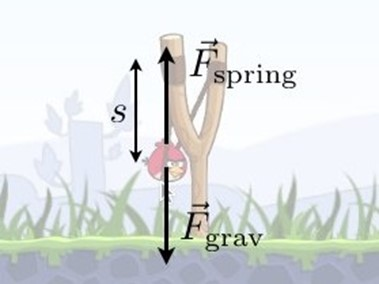
\includegraphics[scale=1.3]{Picture1.jpg} 
    \caption{"Angry Bird stretched on a slingshot"}
 \label{fig:FIG1}
\end{figure}

Figure \ref{fig:FIG2}  displays a bird from 'Angry Birds' in a slingshot, with notations for the stretch distance (s), the launch angle $\theta$, and the vertical height (h) to conceptualize the physics of projectile motion.



\begin{figure}[!h]
    \centering
    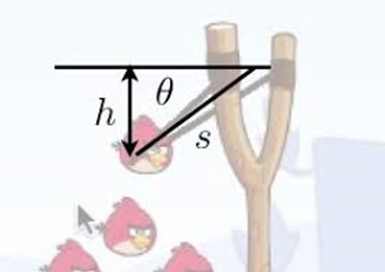
\includegraphics[scale=1]{Picture2.jpg} 
    \caption{Physics of projectile motion for a slingshot}
    \label{fig:FIG2}
\end{figure}

\vspace{2cm}
Figure \ref{fig:FIG3} demonstrates a physics problem using 'Angry Birds', showing a bird being launched from a slingshot at an angle with initial velocity vo, aiming to hit targets A and B placed at different heights and distances.

\begin{figure}[!h]
    \centering
    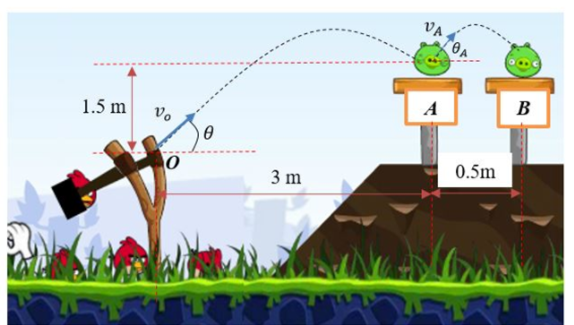
\includegraphics[scale=1]{Picture3.png} 
    \caption{Slingshot Aimed at targets A and B}
    \label{fig:FIG3}
\end{figure}

\newpage

\subsection{Collision}

\begin{figure}[!h]
    \centering
    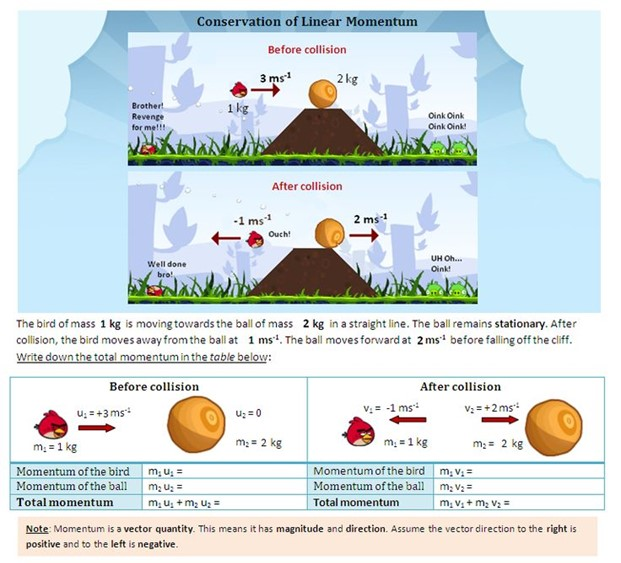
\includegraphics[scale=1]{Picture4.jpg} 
    \caption{Caption provided in image}
    \label{fig:FIG4}
\end{figure}

\begin{figure}[!h]
    \centering
    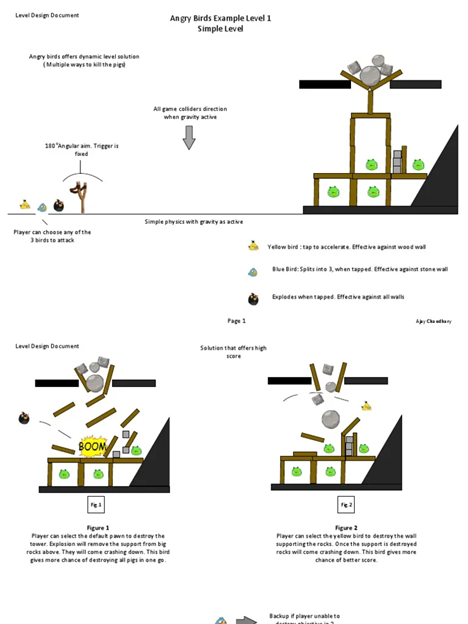
\includegraphics[scale=0.89]{Picture5.png} 
    \caption{Caption provided in image}
    \label{fig:FIG5}
\end{figure}

\end{document}
